\section{The PSP on LHCONE}

The PSP as described works well for single network links, with a single divisible item auctioned among several bidders. However, LHCONE is a far more complex beast, as can be seen in figure~\ref{fig:lhcone}.

\begin{figure}[h]
 \centering
   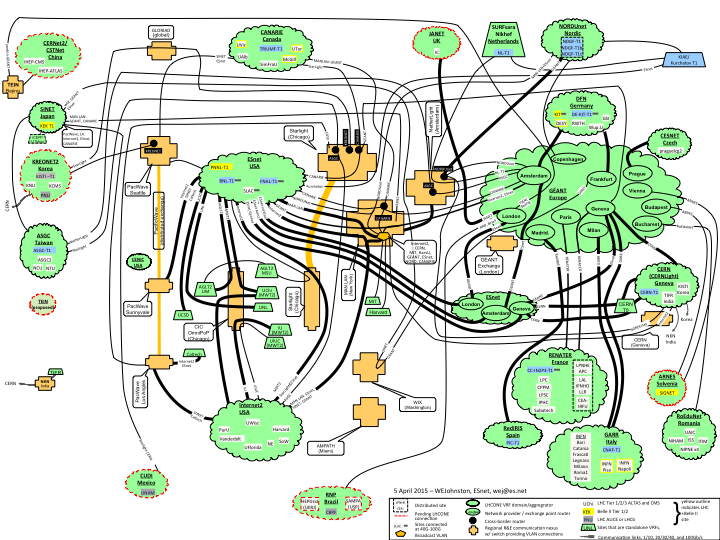
\includegraphics[width=0.8\textwidth]{LHCONE}
       \caption{An approximate schematic of the LHCONE network links, showing the complexity of the LHCONE layout.}
 \label{fig:lhcone}
\end{figure}

Fortunately, the PSP extends naturally to multiple links, where different bidders are interested in different network paths of the network. A full analysis is shown in \cite{PSP-multi}. The PSP properties are maintained by holding multiple independent auctions for each network link. Bidders have a global budget each, which again can vary from bidder to bidder, from which they bid on each of the links that they are interested in in parallel. The optimal strategy for a bidder is to bid for the same bandwidth on each link-segment of the network path they are interested in, varying the price they bid at each segment in accordance with the competition for that link. Convergence to an \textepsilon-Nash equilibrium is still guaranteed for rational bidders, making the PSP a viable candidate for addressing the problem of sharing bandwidth at LHCONE.

One issue that may arise in a complex topology like LHCONE is the existence of multiple paths between endpoints. Whether these are presented to the user as multiple routes on which they must bid, or are hidden inside the LHCONE representation, is an implementation detail, albeit a significant one. If the user is expected to bid on multiple paths for the same traffic then they obviously have a much more complex situation to handle, one which they would probably prefer not to have to deal with. On the other hand, if LHCONE attempts to hide the details of multi-path routing from the user, the maximum bandwidth available between any given pair of endpoints may not be constant, depending on other users on some of the paths.